\chapter{Visualizaci?n y representaci?n de datos espaciales. }


\pagestyle{fancy}

Visualizar la informaci?n geogr?fica es una parte fundamental del trabajo con un SIG. Aunque algunos datos incluyen su propia manera de representarse ---por  ejemplo, las im?genes de sat?lite, las ortofotos, o las obtenidas de un servicio de mapas---, en el SIG es en general el usuario quien define la forma de representar el dato. Es decir, el usuario de SIG \textbf{toma el papel del cart?grafo}, y por tanto debe conocer los fundamentos que este utiliza para la creaci?n de mapas.

Adem?s de las herramientas y conceptos cartogr?ficos cl?sicos, los SIG incorporan elementos de la denominada \textbf{visualizaci?n cient?fica}, tales como la \textbf{interactividad} o la \textbf{representacion de datos multidimensionales}. El resultado de este nuevo planteamiento, m?s rico que el de la cartograf?a cl?sica, se conoce como \textbf{geovisualizaci?n}. 

En este cap?tulo veremos las ideas fundamentales sobre la visualizaci?n de datos, desarrollando la aplicaci?n de estas en la cartograf?a tradicional, as? como en el ?mbito de la geovisualizaci?n y de los SIG.


\section{Conceptos b?sicos de visualizaci?n}

Cuando visualizamos cualquier tipo de informaci?n geogr?fica, ya sea a trav?s de un mapa cl?sico o de alg?n elemento gr?fico en la pantalla de un ordenador, estamos utilizando un \textbf{lenguaje visual} para transmitirla. Del mismo modo que al hablar empleamos un lenguaje oral y al escribir un lenguaje escrito, siempre que plasmemos la informaci?n geogr?fica en una serie de elementos visuales estaremos empleando este lenguaje visual.


El estudio de los signos de un lenguaje constituye lo que se conoce como \textbf{semiolog?a}. En el caso de los elementos del lenguaje visual, encontramos una \textbf{semiolog?a gr?fica}. Esta semiolog?a trata los signos del lenguaje visual y la gram?tica de estos, definiendo una ling??stica visual que nos ayuda a comprender c?mo una representaci?n gr?fica dada cumple su prop?sito de transmitir la informaci?n en base a la cual se crea.


\subsection{Las variables visuales}

Existen diversas propiedades de los elementos visuales que podemos emplear para trasnmitir una informaci?n, siendo m?s adecuadas unas u otras seg?n sea la circunstancia.

\begin{figure}[!hbt]
\centering
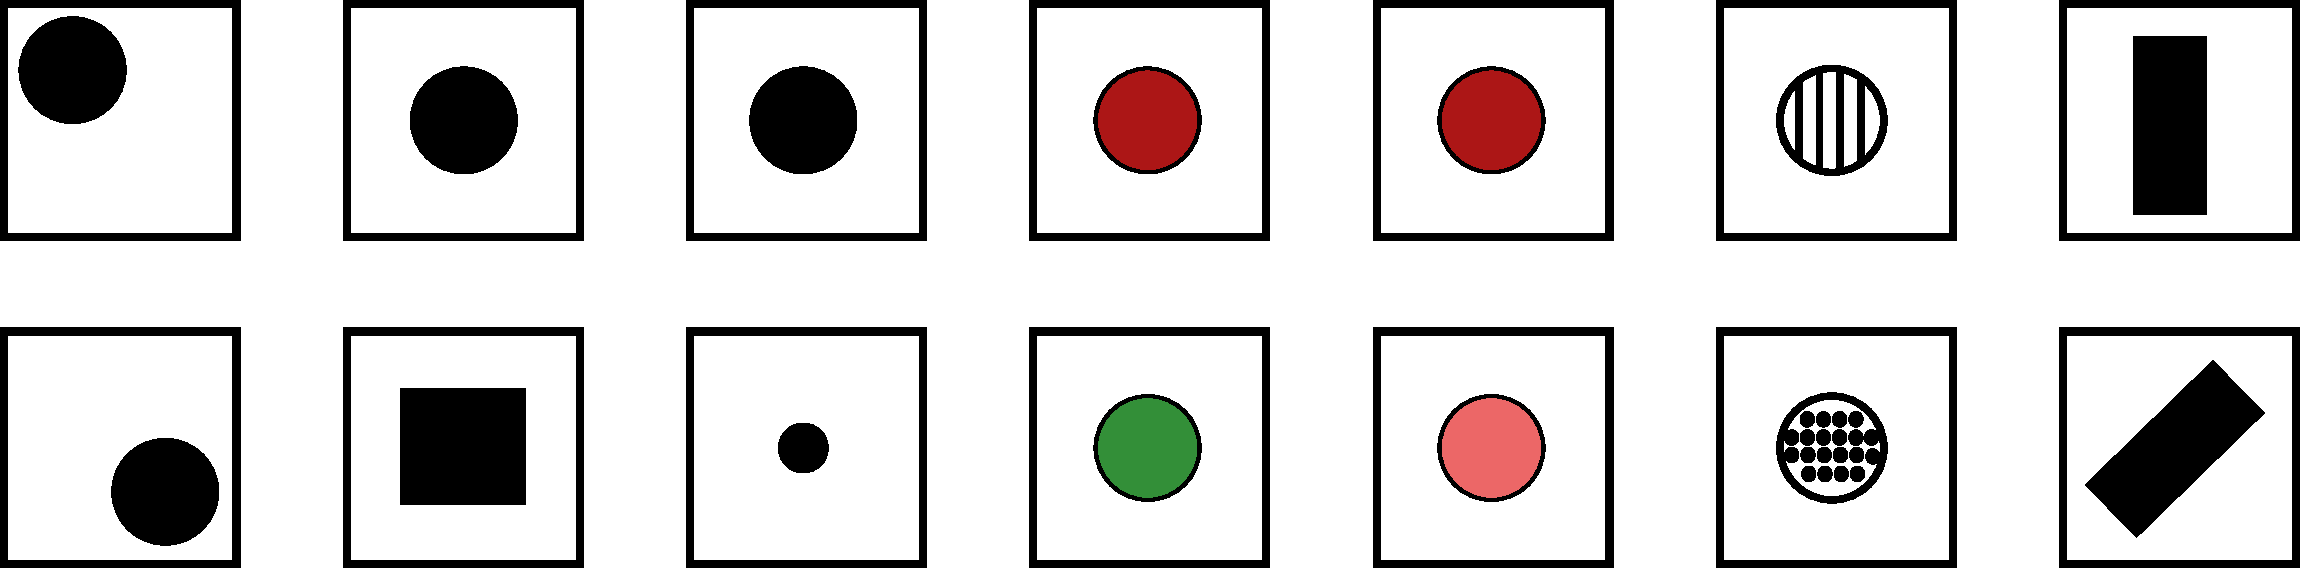
\includegraphics[width=\columnwidth]{../es/Visualizacion/VariablesVisuales.pdf}
\caption{\small Ejemplo de uso de las distintas variables visuales. De izquierda a derecha: posici?n, forma, tama?o, tono, valor, textura, y orientaci?n}
\label{Fig:VariablesVisuales} 
\end{figure}


Estas propiedades conforman lo que se conoce como \textbf{variables visuales}, y se aplican a los elementos b?sicos de la representaci?n, que son aquellos objetos geom?tricos de que se compone esta. Las variables visuales permiten diferenciar unos de otros y asignarles unas ciertas caracter?sticas, susceptibles a su vez de ser interpretadas junto al propio significado que el objeto pueda tener. Dados dos elementos, estos pueden diferenciarse por las siguientes variables, que aparecen representadas en la figura \ref{Fig:VariablesVisuales}: Posici?n, forma, tama?o, textura, color y orientaci?n

El uso de la \textbf{posici?n} est? muy restringido en el caso de un mapa, por deber respetarse el emplazamiento real en el espacio del elemento representado, y por ello y no se emplea.

La \textbf{forma} viene definida por el per?metro exterior del objeto. La forma se aplica fundamentalmente a los s?mbolos puntuales, situando un s?mbolo de una forma dada sobre las coordenadas exactas del punto a representar. Su aplicaci?n a s?mbolos lineales es dif?cil y no se da, mientras que en el caso de aplicarse sobre s?mbolos de superficie requiere la alteraci?n de los pol?gonos representados (por ejemplo, que tracen los l?mites de pa?ses), dando lugar a una representaci?n imprecisa, al menos en lo que al contorno del pol?gono respecta. 

El \textbf{tama?o} se refiere a la dimensi?n del s?mbolo. Para el caso de s?mbolos puntuales, puede aplicarse sin m?s que hacer m?s grande o peque?o el s?mbolo en s?. En el caso de l?neas, el grosor de estas constituye la forma de aplicar la variable tama?o. No se usa en s?mbolos superficiales, salvo aplic?ndolo sobre la textura de relleno.

El tama?o \textbf{condiciona la percepci?n de otras variables visuales}, especialmente cuando se trata de tama?os peque?os. 

La \textbf{textura} hace referencia al relleno de un s?mbolo mediante alg?n patr?n. Se aplica en lineas mediante el uso de guiones y espacios en blanco que dan lugar a un patr?n de discontinuidad, aunque su uso principal es en el caso de s?mbolos de superficie.

El \textbf{color} es la m?s importante de todas las variables visuales, debido a las posibilidades que ofrece.

Dos son las componentes de un color que se utilizan como variables visuales, y que pueden entenderse como tales por si mismas: el tono y el  valor. 

El \textbf{tono} es lo que en el lenguaje com?n denominar?amos color, es decir el nombre del color, por ejemplo verde, rojo o amarillo. 

El tono puede verse \textbf{alterado por los tonos del entorno}, especialmente en s?mbolos de peque?o tama?o. Aunque es una variable para la que la percepci?n humana tiene gran sensibilidad, en los s?mbolos peque?os puede ser dif?cil de identificar y pueden producirse una falsa percepci?n si comparten espacio con otras m?s grandes de un tono distinto. 

Por su parte, el \textbf{valor} indica la claridad del color. Un tono azul puede ser m?s claro o m?s oscuro sin dejar de ser azul. Esa variaci?n que se produce es una variaci?n del valor del color. 

La capacidad de diferenciar dos s?mbolos con valor distinto var?a en funci?n del tipo de s?mbolo. As?, es mayor en el caso de s?mbolos de superficie, mientras que en el caso de s?mbolos puntuales y lineales est? relacionada con el tama?o. Si el punto es muy peque?o o la l?nea muy delgada, es m?s dif?cil apreciar el valor y, por tanto, comparar este con otro o extraer la informaci?n que mediante esa variable visual se intenta transmitir.


Por ?ltimo, la \textbf{orientaci?n} se aplica sobre los s?mbolos puntuales, siempre que estos no presenten simetr?as que impidan percibir correctamente la orientaci?n. Para los s?mbolos de superficie, se aplica a trav?s de la textura, variando la orientaci?n de esta. No se aplica en el caso de l?neas.

\subsection{Las propiedades de las variables visuales}

Se distinguen 4 propiedades b?sicas que una variable visual puede presentar:

\begin{itemize}
	\item \textbf{Asociativa}. Una variable visual presenta la propiedad asociativa si al ser aplicada no aumenta ni disminuye la visibilidad de un elemento. Es decir, cuando en funci?n de esa variable visual no puede asign?rsele m?s o menos importancia a este.
	\item \textbf{Selectiva}. La propiedad selectiva la presentan aquellas variables visuales que, al ser aplicadas, generan distintas categor?as de s?mbolos.
	\item \textbf{Ordenada}. Cuando una variable visual puede emplearse para representar un orden, se dice que presenta la propiedad ordenada.
	\item \textbf{Cuantitativa}. Cuando, adem?s del orden, una variable puede mostrar cantidades o proporciones, entonces se dice que posee la propiedad cuantitativa.
\end{itemize}

En la anterior lista, las propiedades est?n organizadas seg?n los denominados \emph{niveles de organizaci?n}. La propiedad asociativa se sit?a en el nivel m?s bajo, mientras que la cuantitativa ocupa el m?s alto. El nivel de organizaci?n de las variables visuales tiene importancia a la hora de combinar varias de ellas en un s?mbolo, como veremos m?s adelante. Asimismo, el nivel de organizaci?n define qu? tipo de informaci?n podemos transmitir con una variable visual.

La figura \ref{Fig:PropiedadesVariablesVisuales} muestra diferentes representaciones de un conjunto de s?mbolos puntuales en los que en cada caso se ha utilizado ?nicamente una variable visual.

\begin{figure}[!hbt]
\centering
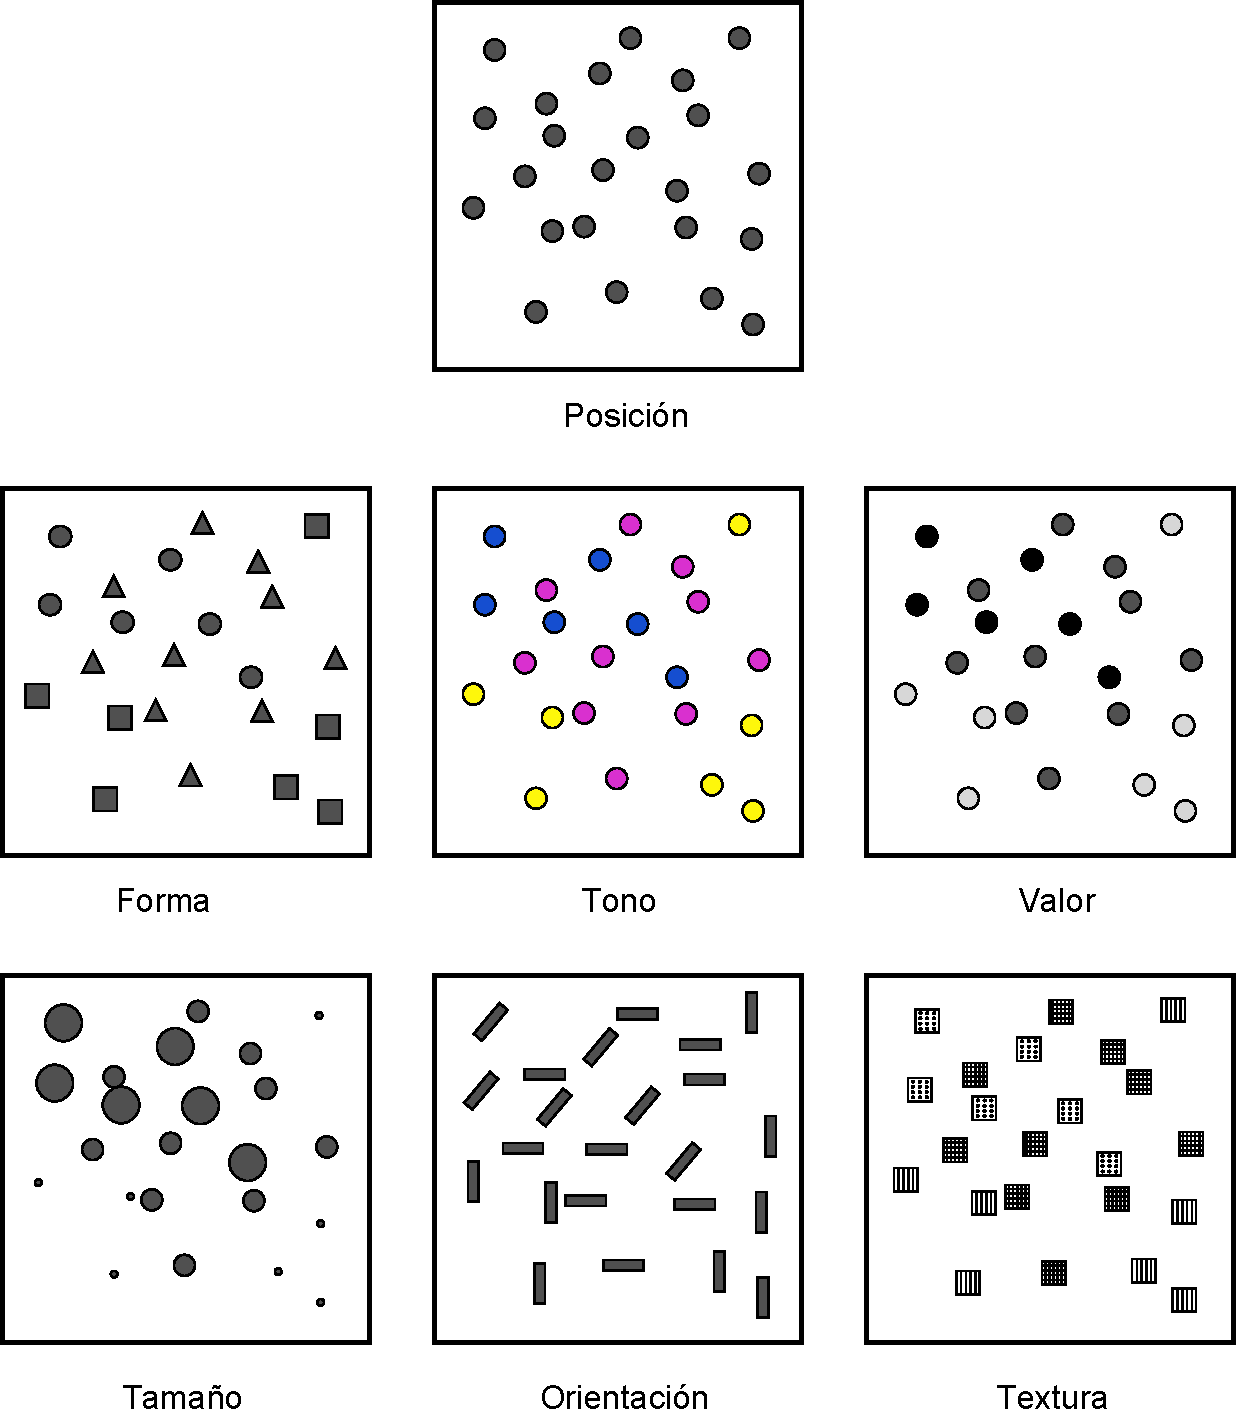
\includegraphics[width=\columnwidth]{../es/Visualizacion/PropiedadesVariablesVisuales.pdf}
\caption{\small Representaci?n de un conjunto de s?mbolos aplicando de forma individual las distintas variables visuales.}
\label{Fig:PropiedadesVariablesVisuales} 
\end{figure}

Comenzando con la propiedad asociativa, vemos que a excepci?n del tama?o y el valor, las dem?s variables visuales no hacen que los elementos presenten una preponderancia en la imagen. No existen una orientaci?n que podamos definir como m?s importante, ni tampoco un color. Lo mismo sucede con la textura, la forma y la posici?n. 

Con el tama?o, sin embargo, resulta claro que mayor tama?o implica un papel destacado dentro de la informaci?n que transmite el mapa. De igual modo, un mayor valor (un color m?s oscuro) da sensaci?n de mayor definici?n, y centra la atenci?n de observador sobre el elemento de un modo muy superior a como lo hace un valor bajo.

Respecto a la propiedad selectiva, diremos que una variable visual la presenta si de un vistazo podemos r?pidamente seleccionar los elementos que pertenecen a un determinado grupo, identificados estos mediante dicha variable visual. El caso m?s claro de propiedad selectiva lo presenta el tono. Podemos r?pidamente quedarnos solo con los elementos amarillos o con los rojos. Aunque no de un modo tan claro, todas las restantes variables presentan igualmente esta propiedad, a excepci?n de la forma. La forma no permite que los elementos se agrupen de modo espont?neo en familias, y su validez en este sentido est? muy ligada a la complejidad de dicha forma.

La propiedad ordenada la presentan aquellas variables que permiten establecer un orden. Tan solo posici?n, textura, tama?o y valor la presentan, mientras que las dem?s carecen de ella. Por ejemplo, en la imagen correspondiente a la variable visual tono no podemos decir cu?les de los elementos situar?amos al principio y cu?les al final de una escala dada definida por esos tonos. Con el valor, sin embargo, s? que podemos, ya que esta escala ir?a de los tonos m?s claros a los m?s oscuros, y visualmente podemos sin dificultad distinguir los distintos niveles y ordenarlos.

Por ?ltimo, la propiedad cuantitativa la presentan aquellas variables visuales que permiten estimar proporciones o cantidades de forma visual. Esta propiedad es exclusiva del tama?o y de la posici?n, mientras que las dem?s no la presentan. Podemos por, ejemplo ver que los c?rculos grandes en la figura correspondiente son aproximadamente el doble que los peque?os. 

En el cuadro \ref{Tabla:PropiedadesVariablesVisuales} se muestra un resumen de todo lo anterior.

% \begin{table}[!hbt]
% \small
% \centering  \label{Tabla:PropiedadesVariablesVisuales}
% \begin{tabular}{p{3.6cm}ccccccc}  
%  & \rotatebox{90}{\textbf{Posici?n}} & \rotatebox{90}{\textbf{Tama?o}} & \rotatebox{90}{\textbf{Forma}} & \rotatebox{90}{\textbf{Valor}} & \rotatebox{90}{\textbf{Tono}} & \rotatebox{90}{\textbf{Textura}} & \rotatebox{90}{\textbf{Orientaci?n}} \\ \midrule   
% \textbf{Asociativa}& $\diamondsuit$ & - & $\diamondsuit$ & - & $\diamondsuit$ & $\diamondsuit$ & $\diamondsuit$ \\
% \textbf{Selectiva}& $\diamondsuit$ & $\diamondsuit$ & - & $\diamondsuit$ & $\diamondsuit$ & $\diamondsuit$ & $\diamondsuit$ \\
% \textbf{Ordenada}&$\diamondsuit$ & $\diamondsuit$ & - & $\diamondsuit$ & - & - & - \\
% \textbf{Cuantitativa}& $\diamondsuit$ & $\diamondsuit$ & - & - & - & - & -  \\
% \bottomrule \end{tabular}
% \caption{\small Cuadro resumen con las propiedades de las variables visuales.}
% \end{table}

Las variables visuales pueden combinarse (por ejemplo representando elementos con puntos de distinto tama?o y tono). Al hacerlo, deben tenerse en cuenta las propiedades de estas del mismo modo que cuando se emplean de forma individual. Las propiedades a reforzar ser?n aquellas que convengan m?s al tipo de informaci?n representado, y deben presentarlas todas las variables a combinar para que el efecto conjunto sea m?s acusado.


\subsection{La percepci?n de las variables visuales}

La percepci?n de las variables \textbf{puede verse alterada por el medio}. Es importante estudiar esta alteraci?n desde dos puntos de vista: la \textbf{constancia perceptiva} (hasta qu? punto podemos modificar los elementos visuales o su entorno sin que dejen de transmitir su informaci?n y sean confundidos sus caracter?sticas) y las \textbf{ayudas a la percepci?n} (c?mo podemos facilitar que se perciban exactamente como pretendemos)

Entendemos por constancias perceptivas a las propiedades de los objetos cuya \textbf{percepci?n no var?a aunque se produzcan modificaciones}. Por ejemplo, dado un objeto redondo tal como una rueda, si lo miramos en una direcci?n perpendicular aparecer? efectivamente como una forma circular perfecta. Sin embargo, si la miramos desde otro ?ngulo, veremos una forma el?ptica, pero ello no nos lleva a pensar que la rueda en s? no sea ya redonda. Este ejemplo muestra la constancia perceptiva de la forma.

No todas las variables visuales tienen una constancia perceptiva como la anterior. Cuando la percepci?n de un elemento cambia aunque el estimulo no lo haga, en lugar de una constancia perceptiva hablamos de un \textbf{contraste perceptivo}. Los contrastes perceptivos pueden inducir una interpretaci?n err?nea de la informaci?n que pretendemos transmitir, al producirse una percepci?n equivocada.

Las siguientes son algunas de las ideas m?s importantes a tener en cuenta a este respecto a la hora de crear un mapa:

\begin{itemize}
	\item El tama?o es la variable visual que m?s afectada se ve, y el tama?o aparente de un objeto puede variar notablemente si se encuentra rodeado de otros de un tama?o distinto. Es importante tener esto en cuenta a la hora de emplear simbolog?a de elementos puntuales en un mapa.	
	\item El valor se ve igualmente alterado al situar alrededor elementos de distinto valor, especialmente si estos son numerosos.
	\item El tono se ve alterado por la presencia de otros tonos distintos. En un mapa, veremos este efecto al enfrentar el color de un elemento sobre el color del fondo. 
	\item Tonos complementarios puestos juntos pueden crear sensaci?n de vibraci?n en la frontera que los separa.
\end{itemize}

En lo que respecta a las ayudas a la percepci?n, el factor m?s importante en la creaci?n de un mapa es una \textbf{correcta separaci?n entre el fondo y la figura}. Dentro de los distintos elementos o niveles de un mapa (que se corresponder?n en l?neas generales con las capas que se empleen en el SIG para crearlo), se han de emplear las propiedades de las variables visuales para restar importancia visual a aquellas que tengan menos relevancia, y de este modo centrar la atenci?n sobre la informaci?n que se desea transmitir por encima de las dem?s.

Para de aquellas capas que tengan la misma importancia y quieran destacarse en el mapa, es necesario establecer una \textbf{adecuada jerarquizaci?n}. Esta jerarqu?a debe aportar una <<profundidad>> a la informaci?n, de forma que existan niveles en esta y se perciba que algunos elementos est?n por encima de otros. La forma de ordenar las distintas capas en un SIG ya establece un orden, aunque este no es en s? suficiente, y deben utilizarse las variables visuales para enfatizar o no unas o otras capas y la informaci?n que contienen.

Como ejemplo de lo anterior, la figura \ref{Fig:JerarquiaMapa} muestra un ejemplo de como una correcta jerarquizaci?n es fundamental para crear mapas de calidad.

\begin{figure}[!hbt]
\centering
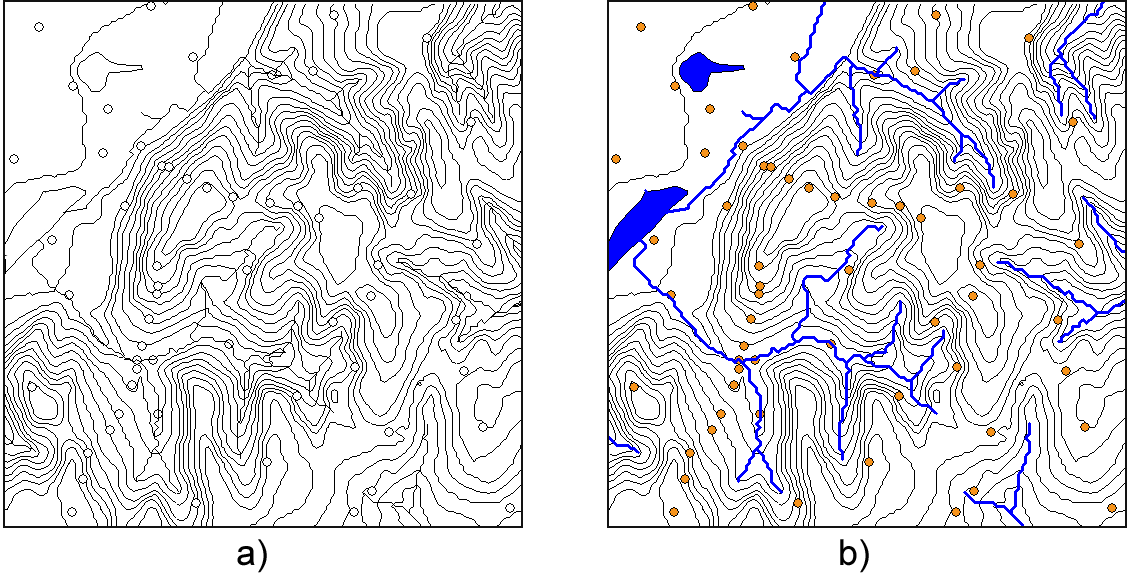
\includegraphics[width=\columnwidth]{../es/Visualizacion/JerarquiaMapa.png}
\caption{\small Mapa con jerarqu?a incorrecta (a) y mapa adecuadamente jerarquizado (b).}
\label{Fig:JerarquiaMapa} 
\end{figure}


\section{El mapa y la comunicaci?n cartogr?fica}

El mapa es un medio de comunicaci?n visual que constituye un lenguaje con un objetivo particular: la \textbf{descripci?n de relaciones espaciales}. Un mapa es, pues, una abstracci?n simb?lica de alg?n fen?meno real, lo cual significa que presenta un cierto grado de simplificaci?n y generalizaci?n.

El lenguaje visual que ya conocemos se convierte ahora en un lenguaje cartogr?fico al adaptarlo al caso particular de la creaci?n de mapas, y sus reglas son imprescindibles para poder crear cartograf?a que facilite la labor posterior del usuario. El conjunto de ideas relativas a la producci?n de mapas dan forma a lo que conocemos como \textbf{dise?o cartogr?fico}.

El dise?o cartogr?fico implica la toma de decisiones por parte del cart?grafo (en este caso el usuario de SIG). Estas decisiones han de estar motivadas fundamentalmente por la \textbf{utilidad del mapa} y el \textbf{p?blico al que va destinado}, y en funci?n de estas han de elegirse aspectos como la \textbf{proyecci?n} a utilizar (no necesariamente la misma en que se encuentran las capas que se van a incluir en el mapa), la \textbf{escala} (dependiendo del nivel de detalle que se desee comunicar, y siempre dentro de las limitaciones de los propios datos), el \textbf{tipo de mapa} (m?s adelante en este cap?tulo detallaremos los tipos m?s importantes), la cantidad de \textbf{simplificaci?n} que debe realizarse o los \textbf{s?mbolos} que han de emplearse para plasmar la informaci?n a transmitir.


Es importante distinguir entre dos tipos de cartograf?a: \textbf{cartograf?a base}, tambi?n denominada \emph{fundamental} o \emph{topogr?fica}, y \textbf{cartograf?a tem?tica}.

La cartograf?a base representa el tipo de mapa que originalmente era el objeto principal de la cartograf?a, cuando lo primordial era recoger con precisi?n \emph{qu?} hab?a sobre la Tierra, documentando a trav?s del documento cartogr?fico las caracter?sticas f?sicas de esta. 

La cartograf?a tem?tica se centra en la \textbf{representaci?n de un tema concreto} (una variable espacial dada), pudiendo esta ser de cualquier ?ndole: f?sica, social, pol?tica, cultural, etc. Se excluyen de la lista de esos temas posibles a los puramente topogr?ficos, que constituyen el objeto de la cartograf?a base.

De otro modo, la cartograf?a topogr?fica representa \textbf{elementos f?sicos del terreno} (un accidente geogr?fico, el curso de un r?o, el perfil de una costa), mientras que la cartograf?a tem?tica se centra m?s en la \textbf{representaci?n de valores y atributos}.

La cartograf?a tem?tica se apoya en la cartograf?a base, ya que esta se incluye tambi?n en los mapas tem?ticos para facilitar la comprensi?n del comportamiento espacial de la variable representada y ubicar esta en un contexto geogr?fico dentro del propio mapa. 


\subsection{Los tipos de informaci?n y su representaci?n}

Sabemos ya que la componente tem?tica de la informaci?n geogr?fica puede ser de tipo num?rico o alfanum?rico, y que la primera se divide en los tipos nominal, ordinal, intervalos y razones.  La selecci?n de una forma de simbolizaci?n adecuada en funci?n de la naturaleza de la informaci?n es clave para lograr un mapa efectivo. En particular, debe emplearse una variable visual que presente la propiedad (nivel de organizaci?n) adecuado. 

Por ejemplo, las propiedades asociativa y selectiva solo son de inter?s para informaci?n cualitativa, mientras que el tama?o es la ?nica variable visual con la propiedad cuantitativa, y por tanto la ?nica adecuada para representar razones.

Las siguientes son algunas ideas b?sicas a este respecto referidas a los distintos tipos antes citados.


\begin{itemize}
	\item \textbf{Nominal}. La informaci?n de tipo nominal se representa adecuadamente utilizando la variable visual forma. Lo que representamos responde principalmente a la pregunta \emph{qu?} en lugar de a la pregunta \emph{cu?nto}, y est? m?s relacionado en cierto modo con la cartograf?a base que con la cartograf?a tem?tica. El uso de s?mbolos, para elementos puntuales o lineales es una soluci?n muy eficaz y habitual en este caso. Para el caso de representar ?reas puede emplearse la variable visual color y emplear distintos tonos, o bien la textura
	
	La informaci?n alfanum?rica se trata a efectos de representaci?n del mismo modo que la de tipo nominal.
	

	\item \textbf{Ordinal}. A diferencia de la informaci?n nominal, en la informaci?n ordinal los valores definen un orden, por lo que la propiedad ordenada es necesaria para poder aplicarla a este caso.
	
	\item \textbf{Intervalos y razones}. Como en el caso anterior, pueden emplearse todas las variables visuales que presenten la propiedad ordenada. No debe olvidarse, no obstante, que la propiedad de mostrar el orden en t?rminos de cantidades o proporciones, que denomin?bamos cuantitativa, es exclusiva del tama?o, siendo este la variable visual m?s adecuada para representar correctamente este tipo de informaci?n.

	Frecuentemente, estos valores son de tipo real (no enteros), por lo que es adem?s necesario agruparlos en clases (intervalos). Esta agrupaci?n puede realizarse seg?n diversas metodolog?as, siendo las m?s habituales los intervalos iguales, los intervalos por percentiles, o los intervalos naturales, que tratan de disminuir la varianza de cada clase.

	El uso de una u otra metodolog?a puede tener un efecto muy notable en la representaci?n, como se muestra en la figura \ref{Fig:TiposIntervalosClases}.

	\begin{figure}[!hbt]
	\centering
	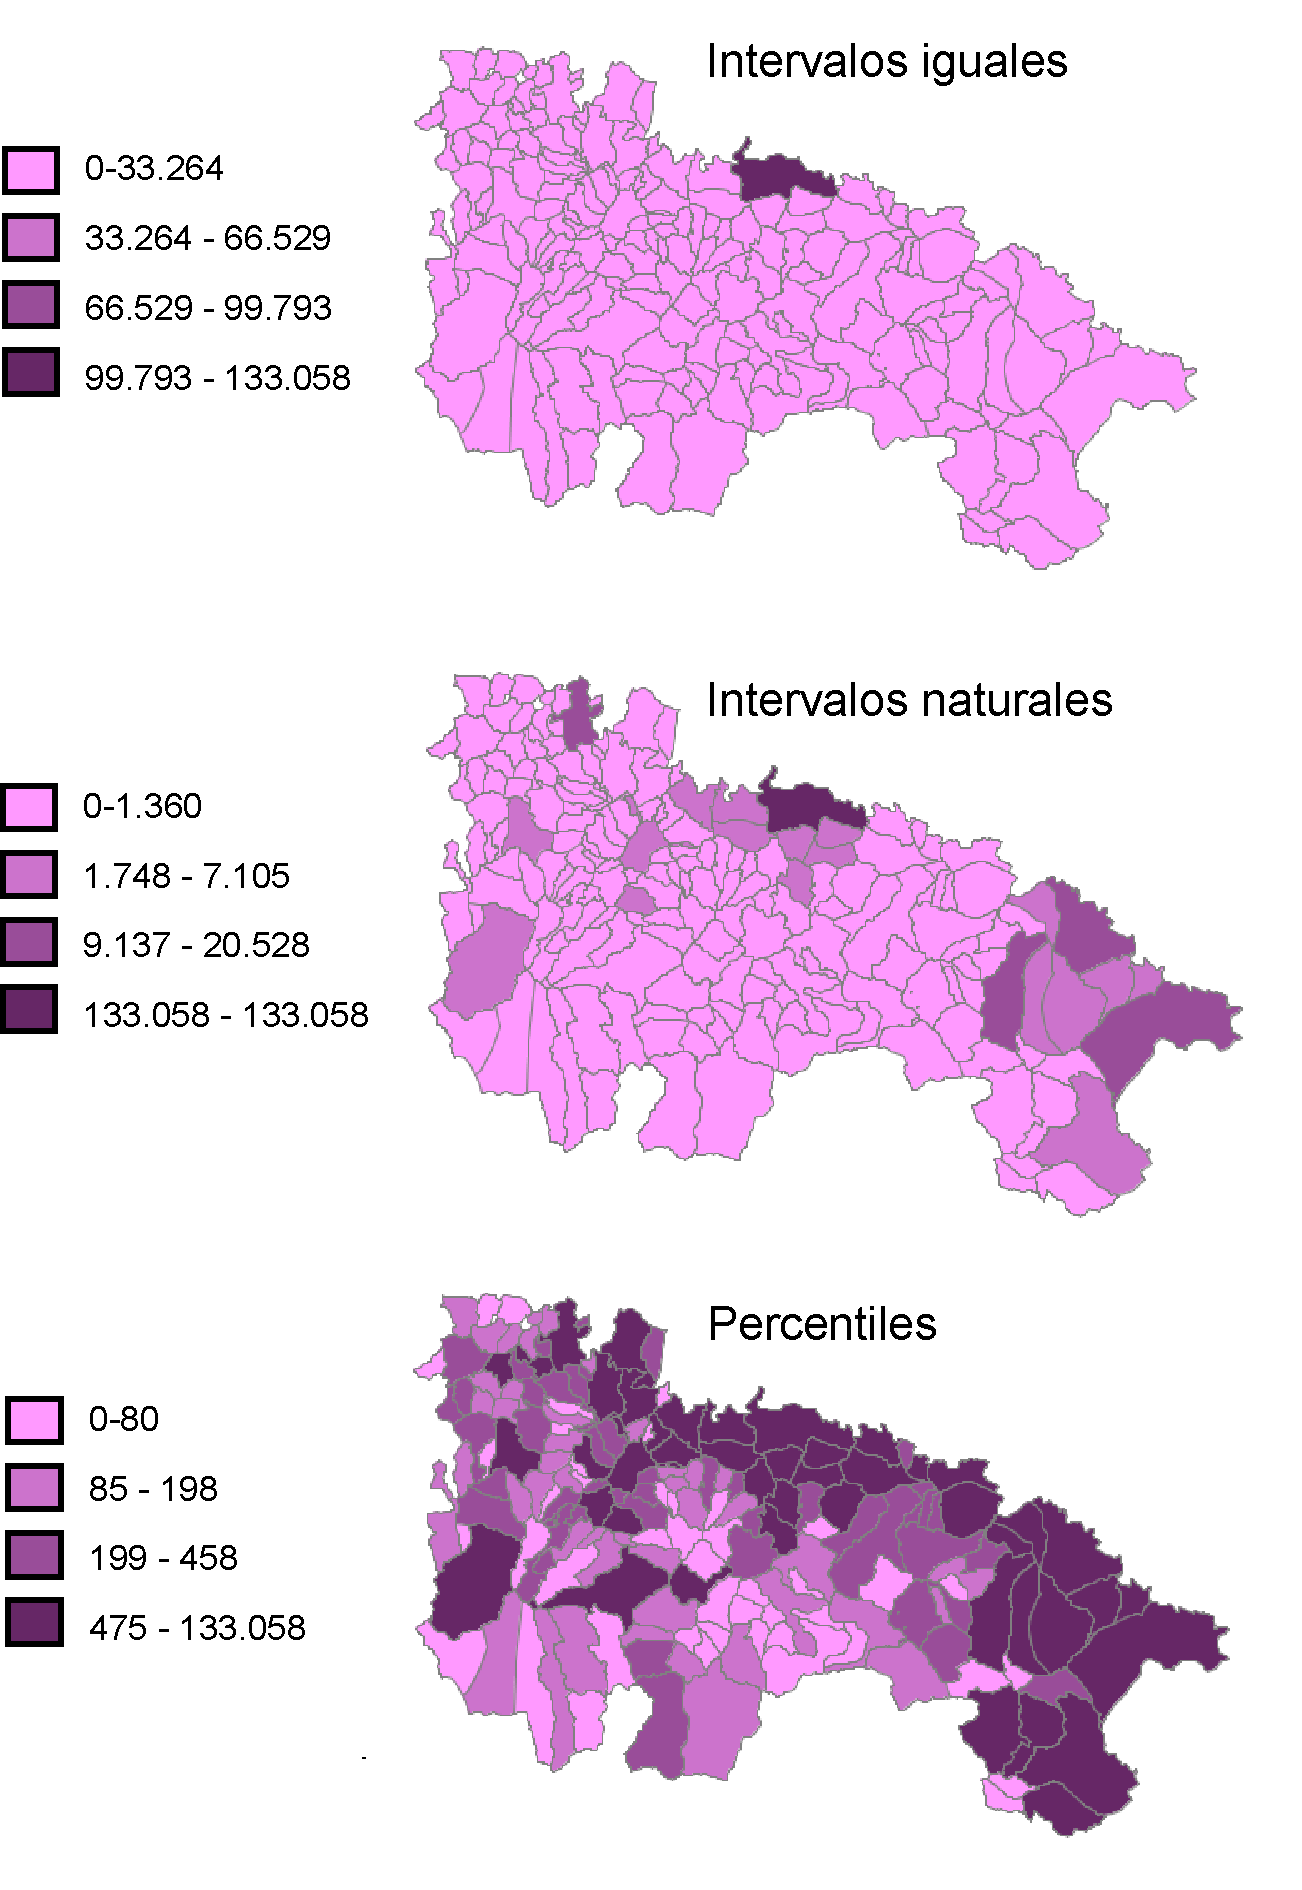
\includegraphics[width=.7\columnwidth]{../es/Visualizacion/TiposIntervalosClases.pdf}
	\caption{\small Comparaci?n entre distintos esquemas para la creaci?n de intervalos de clase.}
	\label{Fig:TiposIntervalosClases} 
	\end{figure}


\end{itemize}


Por ?ltimo, es de inter?s se?alar que, aunque los niveles de organizaci?n de las variables visuales expresan a su vez unas posibilidades crecientes (es decir, con una variable como el valor o el tama?o podemos expresar todo lo que el tono puede transmitir, ya que est?n en un nivel superior), ello no implica necesariamente que el uso de una variable de un nivel superior es mejor que otra de uno inferior. Por ejemplo, el uso del valor para un mapa con informaci?n cualitativa no es adecuado . Puesto que el valor tiene la propiedad ordenada, esto puede inducir a pensar que existe alg?n orden en la variable representada, lo cual es falso. 



\subsection{Elementos del mapa. Composici?n}

Un mapa no es solo lo que se deriva de la representaci?n de la informaci?n geogr?fica y su simbolizaci?n, sino un conjunto de elementos dispuestos de forma ?ptima, siendo uno de ellos aquel que contiene la informaci?n geogr?fica como tal.

Igual de importante que simbolizar correctamente la informaci?n geogr?fica es \textbf{situar adecuadamente los distintos elementos del mapa}, ya que estos est?n pensados tambi?n, al igual que la propia simbolog?a, para facilitar la interpretaci?n de la informaci?n y hacer esta m?s comprensible.

Los siguientes son los elementos fundamentales que podemos emplear para componer un mapa (Figura \ref{Fig:ElementosMapa}):

\begin{figure}[!hbt]
\centering
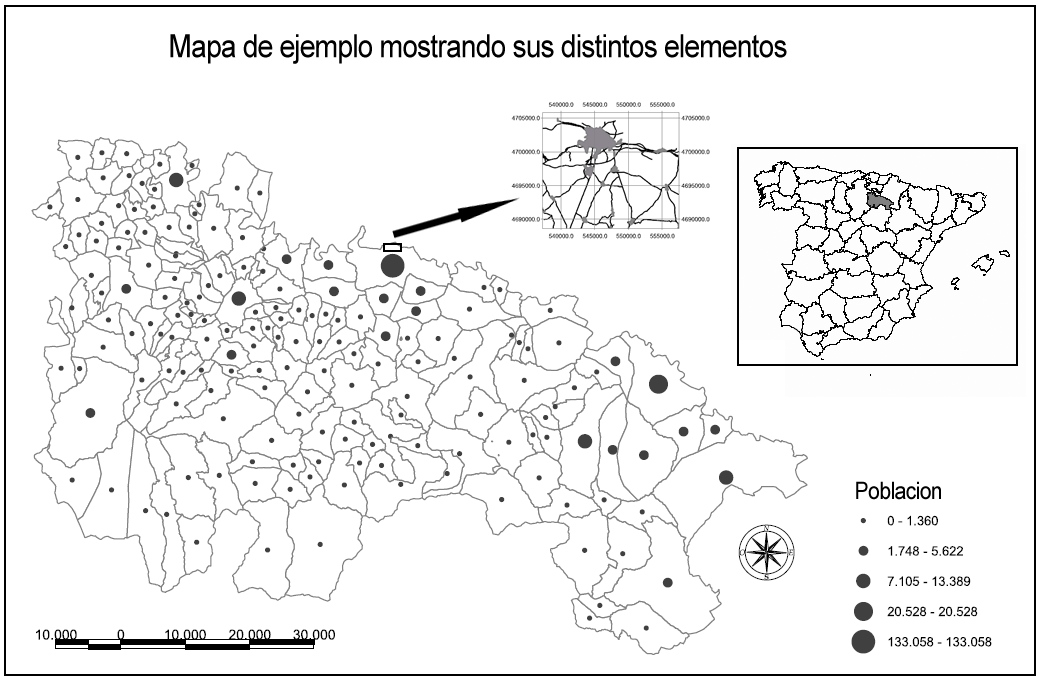
\includegraphics[width=\columnwidth]{../es/Visualizacion/ElementosMapa.png}
\caption{\small Ejemplo de mapa mostrando sus elementos m?s habituales.}
\label{Fig:ElementosMapa} 
\end{figure}

\begin{itemize}
\item \textbf{Nombre o t?tulo}. Imprescindible para conocer qu? informaci?n muestra el mapa.
	\item \textbf{Autor}. La persona u organismo que ha creado el mapa debe aparecer indicada en alg?n punto de este.
	\item \textbf{Otra informaci?n sobre el mapa}. Por ejemplo, la relativa al sistema de referencia empleado o la fecha de su creaci?n, entre otras.
	\item \textbf{Canev?s}. El canev?s es una ret?cula que nos indica d?nde dentro de la superficie terrestre se encuentra aquello que el mapa representa, y provee la referencia geogr?fica para sus elementos. Asimismo, complementa a la escala para la estimaci?n visual de distancias y medidas. Es m?s necesario en caso de escalas bajas, aunque se a?ade con independencia de la escala.
	\item \textbf{Leyenda}. Aunque se ha de tratar de utilizar una simbolog?a lo m?s expresiva posible, no toda la informaci?n puede incorporarse en el mapa, y es necesario acompa?arlo de una leyenda. Esta ha de ser tambi?n f?cil de interpretar y lo m?s clara posible. Una leyenda demasiado extensa o de dif?cil comprensi?n probablemente nos indica que la simbolog?a escogida es mejorable.
	
	
	La leyenda y el mapa en s? forman un todo, por lo que no deben separarse mediante un cuadro, salvo en el caso en que el mapa cubra todo el ?rea del lienzo y no sea f?cil separar visualmente de forma clara ambos elementos.
	\item \textbf{Norte}. Aunque habitualmente se presupone la orientaci?n Norte--Sur, no siempre ha de ocurrir as?, y una aguja apuntando al norte o una rosa de los vientos sirve para aclarar la orientaci?n del mapa. 
	\item \textbf{Escala}. La escala debe indicarse tanto de forma num?rica como gr?fica, de modo que puedan realizarse c?lculos y estimar visualmente distancias entre puntos dados del mapa.\index{Escala}
	\item \textbf{Localizador}. Un localizador provee un elemento visual para situar el mapa en un contexto geogr?fico m?s amplio. Es de especial inter?s en el caso de series de mapas, para establecer la relaci?n entre el presente y los restantes dentro de la misma serie. En este caso, el localizador sirve como mapa ?ndice.
	\item \textbf{Mapas de detalle}. Cuando resulta necesario mostrar una cierta zona del mapa con mayor detalle y a una escala mayor, se puede incluir un mapa correspondiente a esa zona como un enclavado dentro del mapa principal. Se debe se?alar asimismo sobre este ?ltimo la zona a la que corresponde el mapa de detalle.
\end{itemize}



Asimismo, es importante que el dise?o del mapa recalque su prop?sito, haciendo ?nfasis en los aspectos m?s relevantes para cumplir este.


\section{Tipos de mapas tem?ticos}

Existen diversas alternativas en funci?n del tipo de elemento que se pretenda simbolizar o las caracter?sticas de la variable tratada, y la elecci?n de una u otra supondr? una diferencia importante en el mapa obtenido y en su uso posterior. En un mismo mapa pueden combinarse varias de estas formas, especialmente si se pretende representar m?s de una variable, en cuyo caso la combinaci?n debe buscar la m?xima claridad en la representaci?n de todas ellas.

En este apartado detallaremos los siguientes tipos de mapas tem?ticos: mapas de s?mbolos proporcionales, mapas de densidad de puntos, mapas de isol?neas y mapas de coropletas. Todos ellos se utilizan para la representaci?n de variables cuantitativas.


\subsection{Mapas de s?mbolos proporcionales}

Un mapa de s?mbolos proporcionales representa \textbf{variables cuantitativas} a trav?s de s?mbolos cuyo \textbf{tama?o est? en relaci?n con el valor} a representar de dicha variable. Es decir, emplea la \textbf{variable visual tama?o} (la ?nica con la propiedad cuantitativa) para transmitir el valor de la variable representada. Si el s?mbolo es lineal, como por ejemplo una barra, el escalado de los s?mbolos para los distintos valores se realiza utilizando la longitud. Es decir, a un valor doble le corresponde una barra del doble de longitud. En el caso de s?mbolos de superficie, se emplea la superficie. Por ejemplo, en el caso de usar c?rculos, a un valor doble no le corresponde un circulo de radio doble, sino uno de ?rea doble.

El escalado de s?mbolos se puede dar de forma continua, aunque resulta m?s conveniente efectuar un escalado discreto, creando clases y asignando a cada una de ellas un ?nico tama?o. 

Para evitar problemas de percepci?n del tama?o, es importante mostrar en la leyenda la relaci?n entre los distintos tama?os de los s?mbolos y sus valores, como se muestra en la figura \ref{Fig:EjemplosLeyendaSimbolosProporcionales}

\begin{figure}[!hbt]
\centering
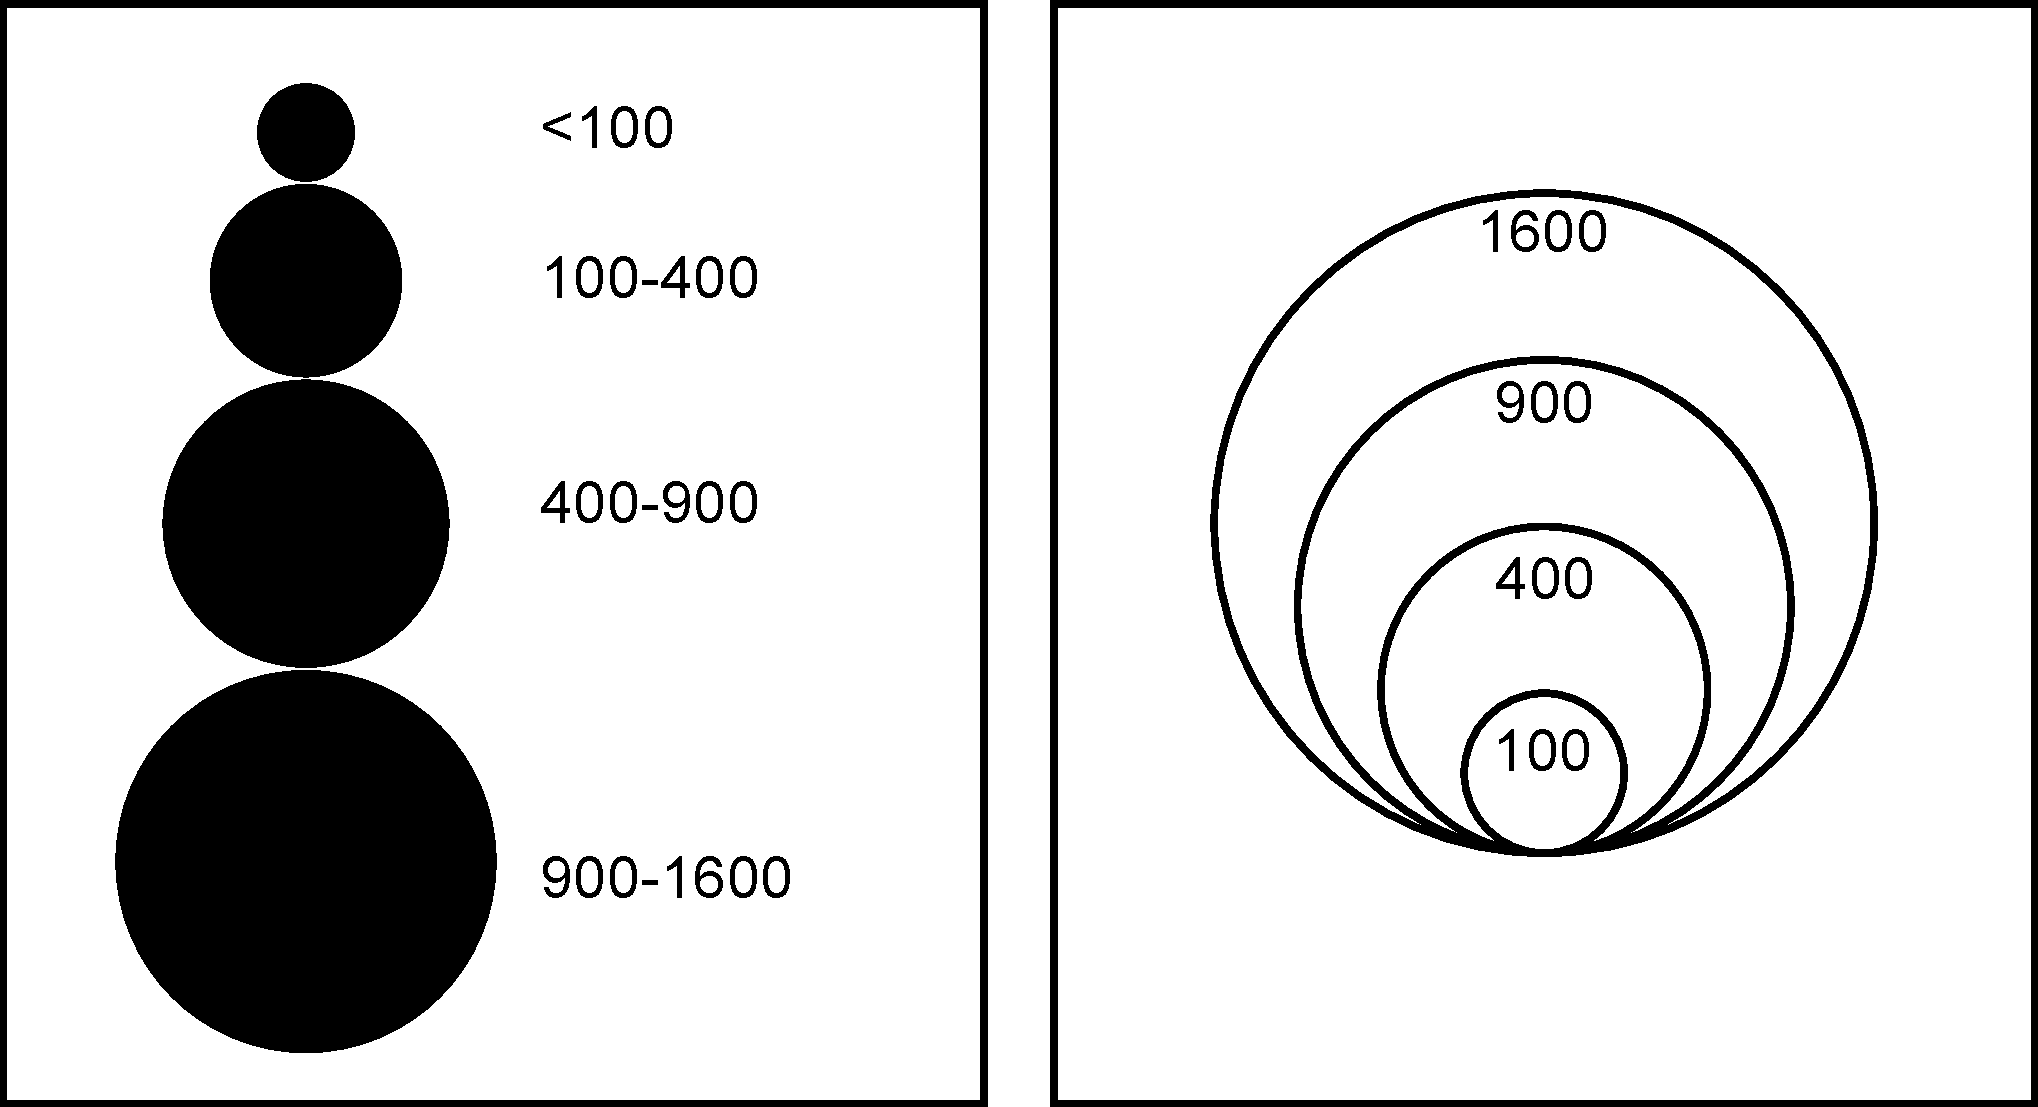
\includegraphics[width=.65\columnwidth]{../es/Visualizacion/EjemplosLeyendaSimbolosProporcionales.pdf}
\caption{\small Dos ejemplos de leyendas para un mapa de s?mbolos proporcionales.}
\label{Fig:EjemplosLeyendaSimbolosProporcionales} 
\end{figure}


\subsection{Mapas de puntos}\index{Mapa!de puntos}

Los mapas de puntos se emplean especialmente para \textbf{variables que representan alg?n tipo de cantidad}, tales como la poblaci?n, el gasto medio por persona o la producci?n de un determinado cultivo. Estas cantidades se representan mediante la \textbf{repetici?n de puntos}, en numero proporcional a su magnitud. Cada uno de esos puntos representa un valor unitario, y el conjunto de ellos sobre la zona en cuesti?n suma la cantidad total a representar. Los puntos tienen todos la misma forma y tama?o, a diferencia de lo que vimos en el caso de los s?mbolos proporcionales. Son especialmente adecuados para variables discretas (valores enteros)

Tres son los aspectos que deben tenerse en cuenta a la hora de elaborar un mapa de puntos: el \textbf{valor de cada punto} (es decir, cu?ntas unidades de la variable representa cada punto), su \textbf{tama?o} y su \textbf{posici?n}.

El valor de cada punto se debe establecer \textbf{en funci?n de los valores m?nimo y m?ximo} de la variable, para que resulte en un mapa en el que los puntos no aparezcan en demas?a o sean demasiado escasos. Este valor se representar? en la leyenda para su interpretaci?n, habitualmente en forma de texto, escribiendo por ejemplo, que <<un punto equivale a 1000 habitantes>>.

La elecci?n del tama?o del punto debe garantizar la buena visibilidad de este, al tiempo que no debe ser excesivamente grande para que no ocupe demasiado espacio y dificulte la visi?n de otros. El \textbf{tama?o ?ptimo est? en relaci?n con el valor unitario} escogido, y ambos par?metros deben establecerse conjuntamente para lograr la combinaci?n m?s adecuada.

La posici?n del punto es de gran importancia para transmitir la informaci?n correcta y no dar lugar ambig?edades o incorporar errores conceptuales. Si no disponemos de informaci?n adicional y solo tenemos el valor correspondiente a una zona dada, los puntos se han de disponer de forma regular ocupando toda la superficie de la zona. Si, por el contrario, sabemos algo m?s acerca de la distribuci?n de la variable, debemos emplear esa informaci?n para emplazarlos de forma m?s realista. Si, por ejemplo, la zona corresponde a una provincia y sabemos la localizaci?n de la principal ciudad dentro de ella, es m?s l?gico situar m?s puntos cerca del emplazamiento de esa ciudad que en otras partes de la provincia, ya que una mayor parte de la poblaci?n estar? all?.

Otro aspecto a considerar es el significado de la variable que se representa y la posibilidad o no de que aparezca en las distintas localizaciones de los puntos. Si la variable es, por ejemplo, el numero de ejemplares avistados de un determinado ave acu?tica, situar los puntos sobre zonas urbanas o de bosque no tiene sentido, ya que dan a entender que ah? hay presencia de esa especie (tantos ejemplares como los puntos en cuesti?n indiquen), algo que es falso.


La imagen \ref{Fig:MapaPuntos} muestra un ejemplo de un mapa de puntos.


\begin{figure}[!hbt]
\centering
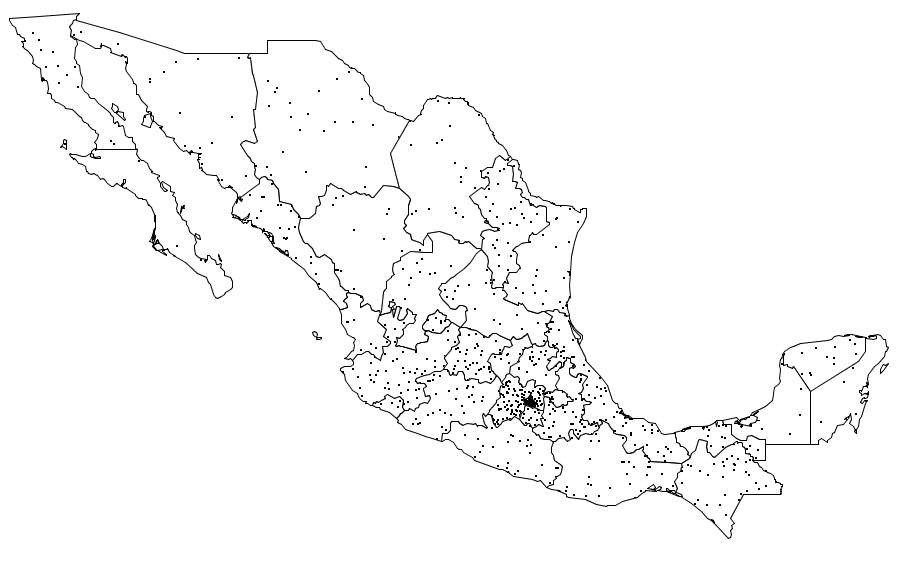
\includegraphics[width=.8\columnwidth]{../es/Visualizacion/MapaPuntos.png}
\caption{\small Mapa de puntos.}
\label{Fig:MapaPuntos} 
\end{figure}


\subsection{Mapas de isol?neas}

Los mapas de isol?neas son muy utilizados para la representaci?n de \textbf{variables continuas}. Se combinan adecuadamente con otros tipos de mapas, ya que, al representarse ?nicamente mediante l?neas, permite la presencia de otros elementos dentro del mapa sin resultar obstrusiva.

Un mapa de isol?neas est? formado por un conjunto de l?neas, cada una de las cuales une \textbf{puntos que presentan el mismo valor} de la variable. Estas l?neas no pueden cruzarse, ya que ello significar?a que en un punto se presentan dos valores. El caso m?s t?pico de mapa de isol?neas son las curvas de nivel que aparecen el un mapa topogr?fico, indicando la elevaci?n del terreno.

La representaci?n de isol?neas viene definida por la denominada \textbf{equidistancia}, que indica la diferencia entre los valores de dos isol?neas contiguas. Una menor equidistancia implica un mayor n?mero de isol?neas y una representaci?n m?s densa.

La variable visual tama?o es la ?nica que suele emplearse para simbolizar isol?neas, en particular para se?alar aquellas l?neas que representan un valor m?ltiplo de una determinada cantidad y hacer as? m?s f?cil la lectura del mapa. Estas l?neas son lo que se conoce como \textbf{curvas directrices}. 

\begin{figure}[!hbt]
\centering
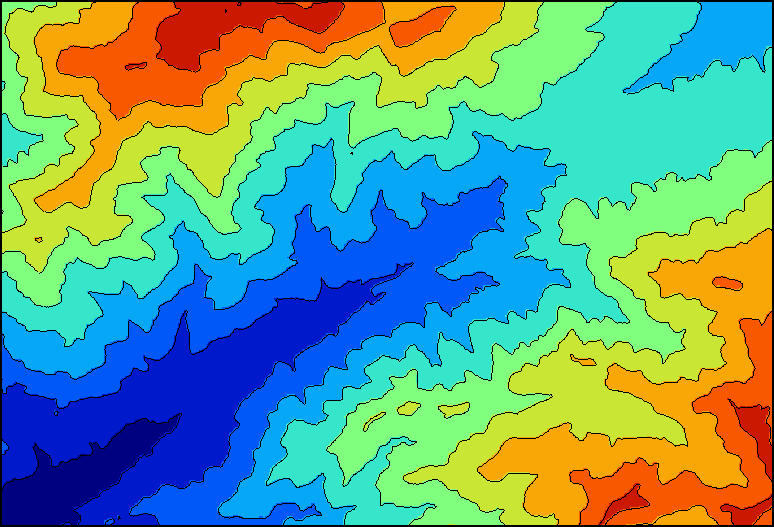
\includegraphics[width=.8\columnwidth]{../es/Visualizacion/Isolineas.png}
\caption{\small Mapa de isol?neas. Se ha empleado para su representaci?n tanto las l?neas como el coloreado de las franjas entre estas.}
\label{Fig:Isolineas} 
\end{figure}


Las l?neas se etiquetan con el valor que representan (con texto sobre la l?nea), y se aprovecha el hecho de que dos l?neas consecutivas est?n separadas siempre por una magnitud igual a la equidistancia, lo cual aporta un importante contexto en lo que a los valores se refiere. 

Una forma particular de representar las isol?neas mediante color es hacerlo no sobre las l?neas, sino sobre las zonas que median entre ellas. Es decir, representar la clase en lugar del l?mite de clase. Este tipo de mapas se asemeja al mapa de coropletas (que veremos seguidamente), trat?ndose m?s de un mapa de ?reas que de l?neas, por lo que se conoce como de \emph{isocoropletas}. Ambos tipos de representaci?n, mediante ?reas y mediante l?neas, pueden combinarse en un ?nico mapa.\index{Isocoropletas}

En la figura \ref{Fig:Isolineas} puede verse un ejemplo de mapa de isol?neas combinando las dos formas anteriores.


\subsection{Mapas de coropletas}\index{Mapa!de coropletas}

Los mapas de coropletas son utilizados habitualmente para representar la informaci?n geogr?fica en un SIG. Por ejemplo, los mapas de la figura \ref{Fig:TiposIntervalosClases} son todos ellos mapas de coropletas.

En un mapa de coropletas se tiene una serie de ?reas definidas, cada una de las cuales posee un valor de una variable. Este valor de la variable afecta a todo el ?rea y es el que se representa por medio de alguna variable visual, normalmente el color a trav?s de su componente valor.

Los mapas de coropletas adolecen de ciertos inconvenientes, siendo los principales la \textbf{sensaci?n de cambio brusco en los l?mites entre ?reas}, la cual puede transmitir la idea de que en esa frontera los valores de la variable cambian bruscamente, ocultando la continuidad de la variable en caso de existir esta,, y la \textbf{homogeneidad dentro de cada ?rea}, que puede no ser cierta.

Para transmitir correctamente la informaci?n, es importante normalizar la variable en funci?n de la superficie de cada unidad. Por ejemplo, en el caso de representar la poblaci?n de una serie de t?rminos municipales, es m?s adecuado representar la poblaci?n por unidad de ?rea, dividiendo el valor de poblaci?n cada unidad entre la superficie de esta.


\section{La visualizaci?n en un SIG}


Una vez que conocemos los conceptos b?sicos sobre representaci?n gr?fica y su uso para la elaboraci?n de mapas, es momento de ver c?mo estos se aplican en el contexto de un SIG. Dos aspectos son especialmente relevantes a este respecto: el hecho de \textbf{contar con m?ltiples capas} que han de representarse conjuntamente, y las \textbf{particularidades de la representaci?n en pantalla}, con la interactividad que el SIG ofrece.


\subsection{Combinaci?n de capas}

En general, una capa aislada no constituye la forma ?ptima de visualizar esta. Si en un mapa encontramos elementos variados, ello no obedece a la mera econom?a de espacio, sino a que a?adir informaci?n adicional a la de esa capa que queremos representar nos ayuda a entenderla mejor. Los procesos que tienen lugar en el espacio est?n relacionados unos con otros, y \textbf{visualizar esas relaciones aporta una mayor riqueza a la visualizaci?n}, haciendo que sea m?s sencillo extraer la informaci?n contenida en ella. 

Aunque sencillo de llevar a cabo en lo que a manejo del SIG respecta, combinar capas es un proceso que tambi?n debe realizarse con conocimiento y en el que, si se realiza correctamente, las diferencias pueden ser notables. No solo se trata de dar espacio dentro del mapa a toda la informaci?n que esas capas contienen, sino que exista una sinergia entre ellas en la medida de lo posible, para que se complementen mutuamente como partes de un conjunto. 


La configuraci?n fundamental en este sentido es el \textbf{orden de las capas}, que indica c?mo se disponen estas las unas sobre las otras y define el orden de pintado. Si una misma zona est? ocupada por elementos de varias capas, solo ser?n visibles los correspondientes a la capa superior, ya que la representaci?n de los pertenecientes a las dem?s quedar? oculta. 

Sabemos que las capas r?ster llenan todo el espacio y contienen valores en todas sus celdas (o p?xeles en el caso de im?genes). Por ello, van a tapar lo que se sit?e por debajo de ellas y no resulta buena idea situarlas en lo alto del orden de pintado. En su lugar, se deben considerar como \textbf{capas base sobre las que situar las restantes}, de tal modo que no impidan a estas visualizarse correctamente.

Con un razonamiento similar, podemos establecer la mejor forma de ordenar las capas vectoriales, situando por norma general los pol?gonos y encima de estos las l?neas y los puntos respectivamente. 


En ocasiones, un determinado orden viene \textbf{impuesto por el significado} que tienen las capas. Por ejemplo, si nuestro mapa contiene una capa con la red de drenaje y otra con carreteras, lo l?gico y habitual es que las carreteras est?n por encima de los r?os, ya que lo normal es que pasen por encima de estos y no al contrario. 


Una funcionalidad de que disponen los SIG para la combinaci?n de capas es el uso de \textbf{transparencias} totales o parciales. Estas se pueden aplicar tanto a capas r?ster como vectoriales, de forma que puede verse a trav?s de ellas y as? presentar la informaci?n de otras capas que se encuentren por debajo. Por ejemplo, la representaci?n mostrada en la figura \ref{Fig:CombinacionCapas} hace uso de esta t?cnica. El pol?gono que delimita la cuenca vertiente es semi--transparente, de tal modo que la capa de relieve sombreado que est? debajo puede verse, dando la sensaci?n de que sigue ese relieve.

\begin{figure}[!hbt]
\centering
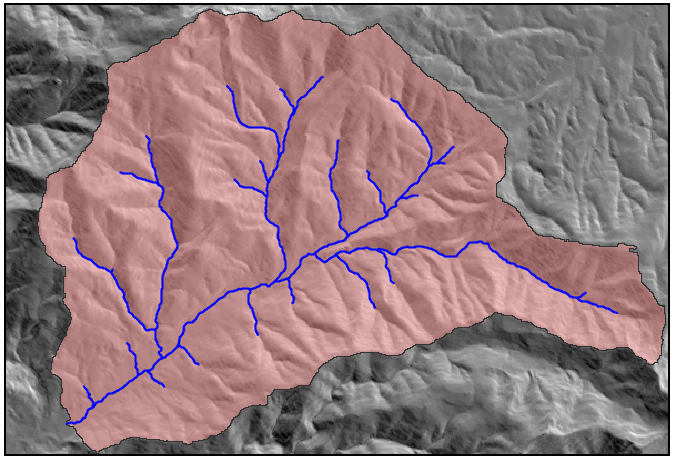
\includegraphics[width=.7\columnwidth]{../es/Visualizacion/CombinacionCapas.png}
\caption{\small Combinaci?n de capas mediante transparencia.}
\label{Fig:CombinacionCapas} 
\end{figure}

En el caso de una capa r?ster, puede aplicarse una transparencia total, haciendo que determinadas partes de esta no se representen, en funci?n de sus valores.

En el caso en que una variable se encuentre dividida en \textbf{varias capas} (divisi?n horizontal), debe asignarse una \textbf{misma simbolog?a} a todas esas capas, con el fin de que la representaci?n sea coherente.


\subsection{Particularidades de la representaci?n en pantalla}

Tanto para las representaciones en papel como para las representaciones en pantalla se siguen unos mismos principios a la hora de dise?arlas, pero estas ?ltimas presentan algunas caracter?sticas particulares que hacen necesario tener en consideraci?n otros factores. 

Podemos distinguir dos bloques fundamentales de diferencias que hacen que un mapa pensado para ser visualizado en la pantalla mientras ejecutamos un SIG no deba dise?arse exactamente igual que si estuviera pensado exclusivamente para ser utilizado en un soporte impreso: la \textbf{baja resoluci?n de la pantalla} y la \textbf{interactividad} de la propia representaci?n.


A la hora de preparar cartograf?a impresa, la resoluci?n no es un problema, ya que las capacidades de que se dispone superan a las necesidades que el cart?grafo puede tener. En la pantalla, sin embargo, algunos elementos pueden no aparecer con suficiente claridad y, aunque en papel cumplan su funci?n correctamente, es conveniente sustituirlos por otros m?s adecuados cuando no se trabaja sobre un medio impreso. Entre los elementos a evitar se encuentran las \textbf{fuentes con ornamentos} tales como sombreados, las \textbf{fuentes con serifas} (peque?os adornos al final de las l?neas para facilitar la lectura) o los \textbf{rellenos o punteados de paso muy fino}.

Respecto a la interactividad de las representaciones, debe tenerse presente que, a diferencia de un mapa impreso, en un SIG lo que vemos no es un elemento est?tico, sino din?mico. En este contexto, \emph{din?mico} no quiere decir que el mapa cambie o que represente un proceso din?mico, sino que el usuario puede alterarlo utilizando por lo menos las herramientas m?s fundamentales que proporcionan interactividad, tales como el desplazamiento, el acercamiento o el alejamiento. 

Por ejemplo, el hecho de que la escala de la representaci?n pueda variar seg?n la voluntad del usuario puede causar problemas con algunos de sus elementos  tales como s?mbolos o etiquetas de texto. Si todos los elementos del mapa se escalan proporcionalmente, una reducci?n importante de escala disminuir? el tama?o del texto hasta hacerlo ilegible. Por el contrario, si aumentamos la escala el tama?o puede ser excesivo. La figura \ref{Fig:ProblemasRepresentacionSimbolos} muestra este hecho. 


\begin{figure}[!hbt]
\centering
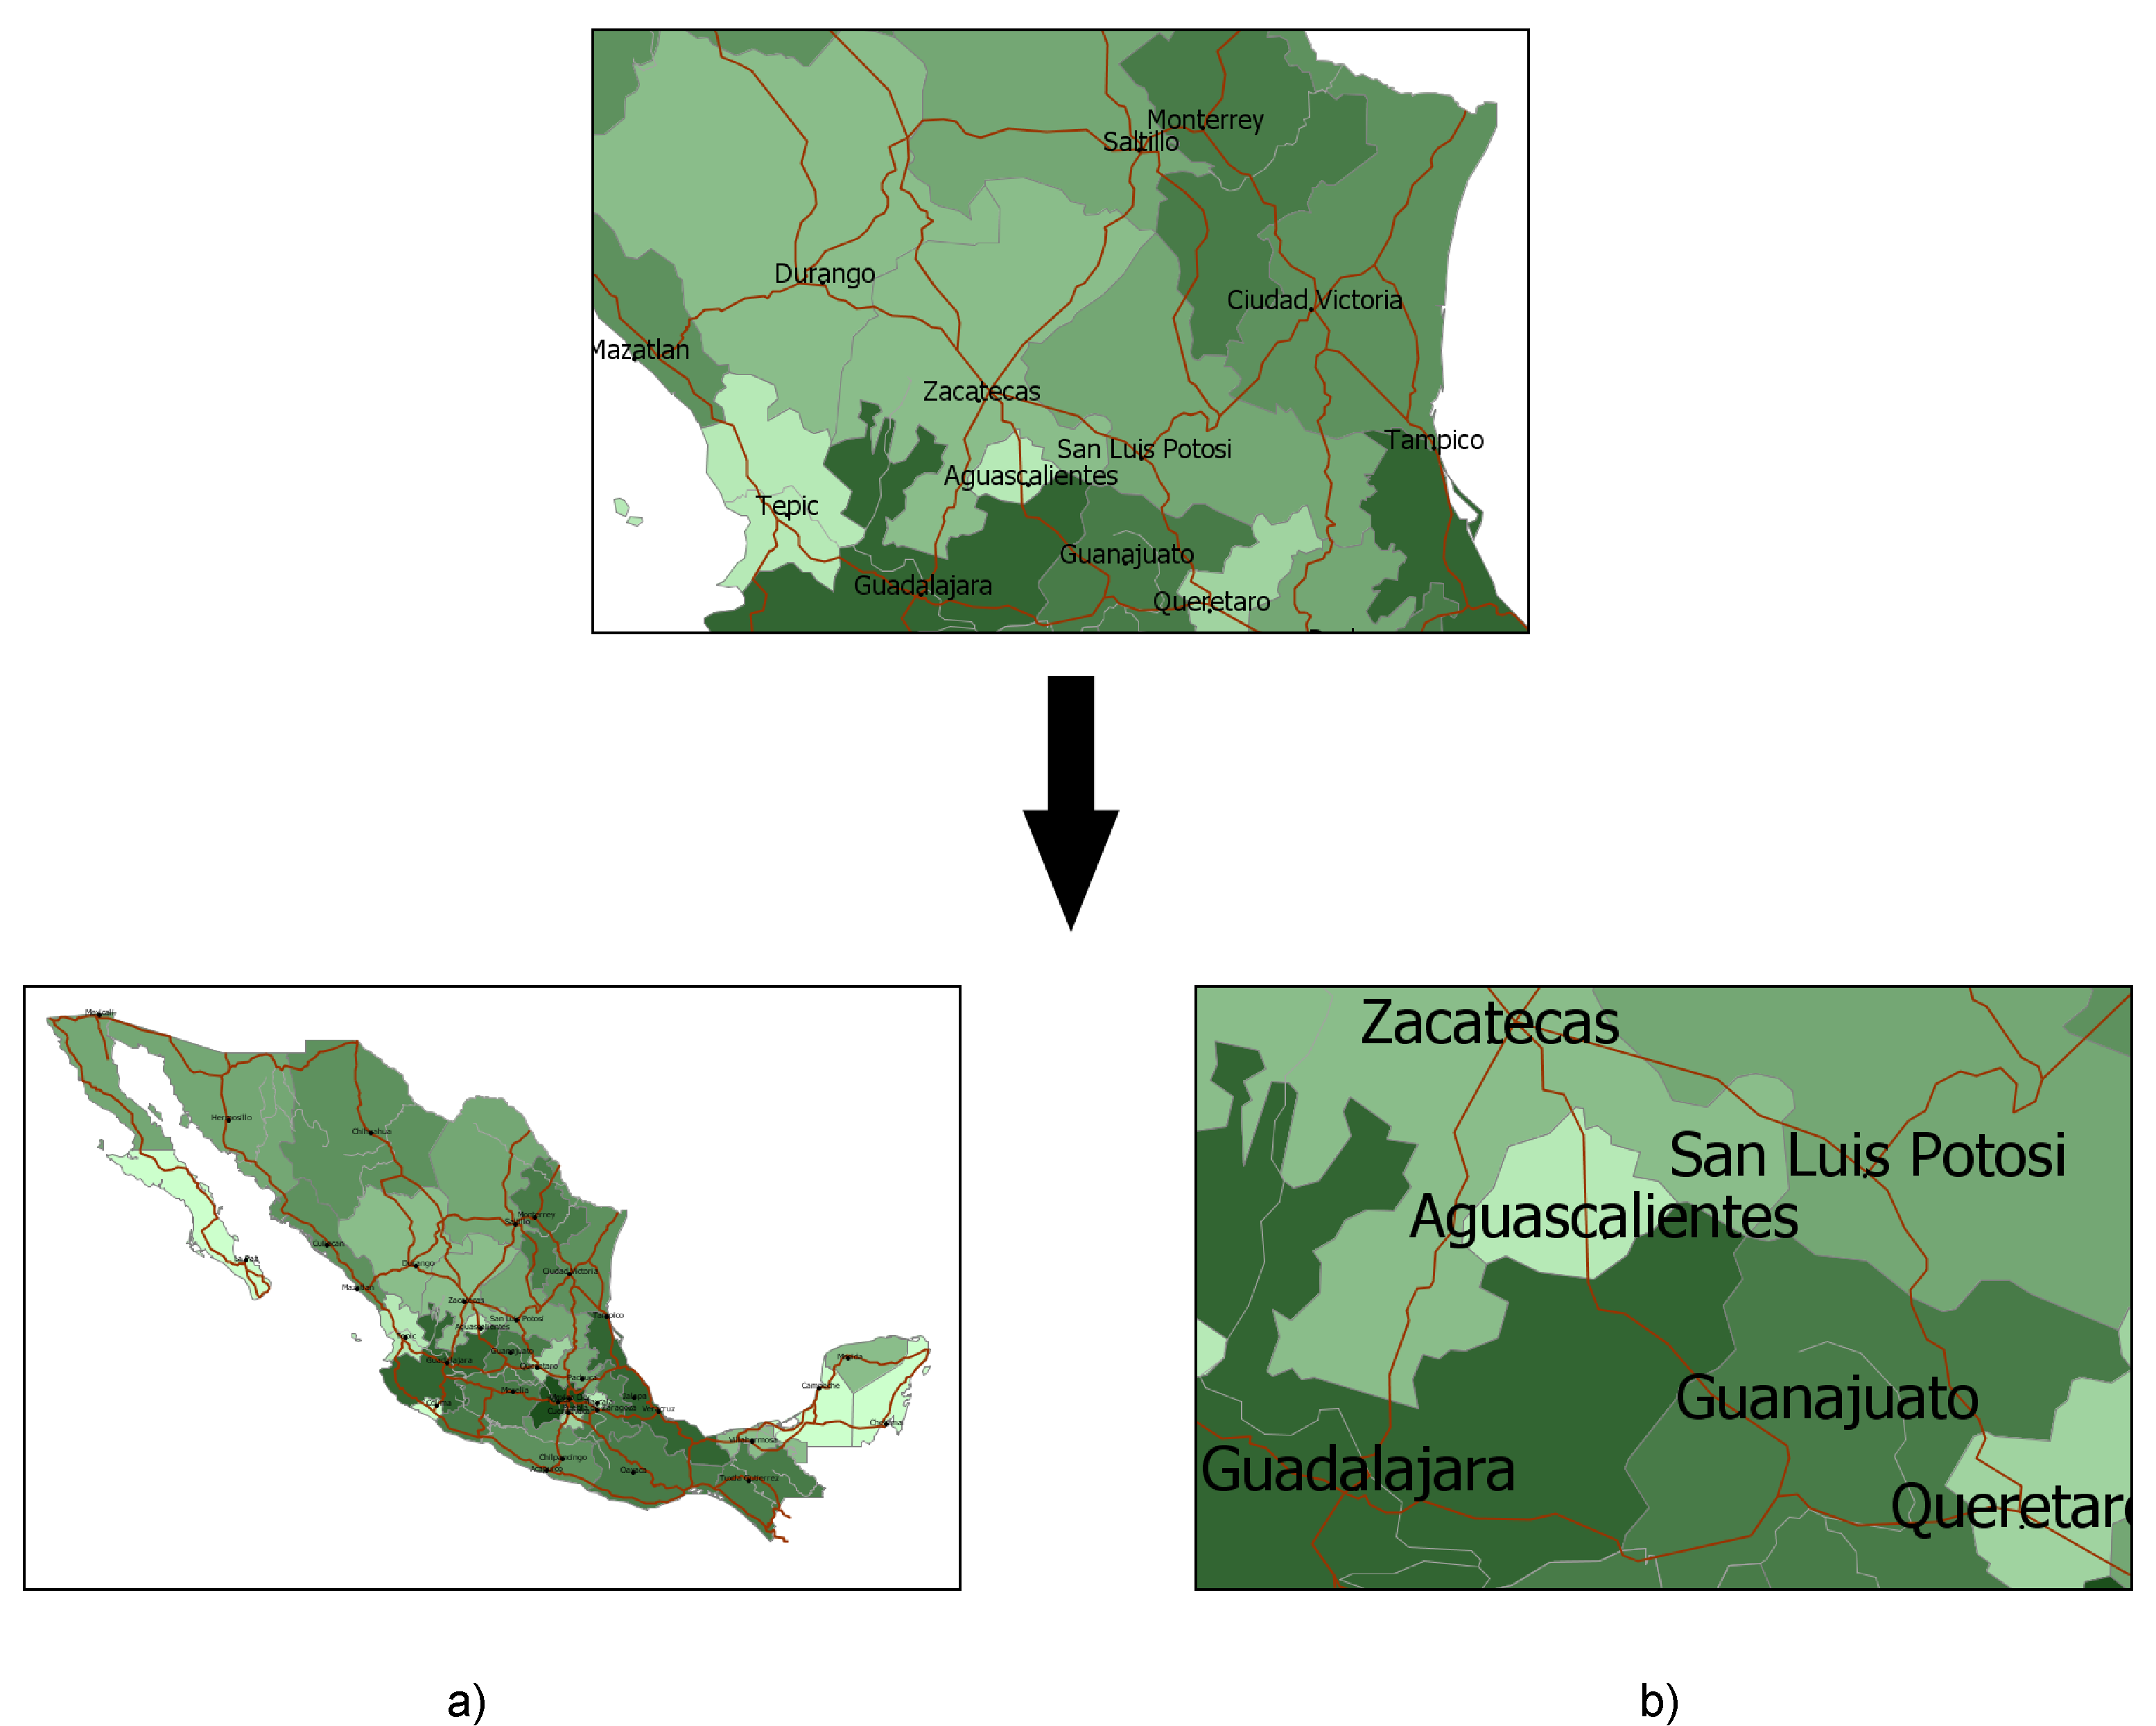
\includegraphics[width=\columnwidth]{../es/Visualizacion/ProblemasRepresentacionSimbolos.pdf}
\caption{\small El cambio de escala var?a el tama?o de los s?mbolos tales como las etiquetas, haci?ndolos demasiado peque?os (a) o demasiado grandes (b)}
\label{Fig:ProblemasRepresentacionSimbolos} 
\end{figure}


Una soluci?n a esto es especificar un \textbf{tama?o absoluto} de estos elementos que no var?e con la escala. Es decir, que un s?mbolo o una etiqueta de texto tengan siempre el mismo tama?o en pantalla y ocupen los mismos p?xeles. A escalas bajas, sin embargo, este m?todo puede dar lugar a representaciones saturadas, como se observa en la figura \ref{Fig:RepresentacionSaturada}.

\begin{figure}[!hbt]
\centering
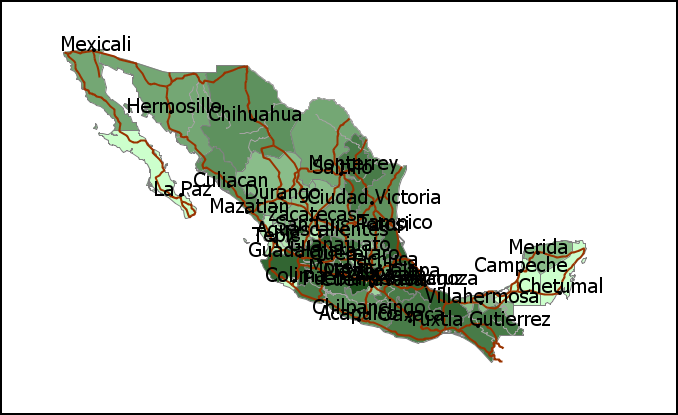
\includegraphics[width=.9\columnwidth]{../es/Visualizacion/RepresentacionSaturada.png}
\caption{\small Representaci?n saturada al representar elementos con tama?o fijo a una escala baja.}
\label{Fig:RepresentacionSaturada} 
\end{figure}

La posibilidad de representar capas a distintas escalas, puede tambi?n dar lugar a \textbf{problemas de rendimiento}. Para evitar estos, se recomienda un \textbf{planteamiento multi--escalar} en el que, seg?n la escala, se visualicen unas u otras capas, as? como trabajar con capas de menor detalle a escalas peque?as

\pagestyle{empty}
